\documentclass[12pt]{letter}

\usepackage[margin=1in,footskip=0.25in]{geometry}

\usepackage{tikz-cd}

\usetikzlibrary{arrows,automata,positioning}

\usepackage{comment}


\begin{document}

Viet Tran Quoc Hoang \\ ID: 01607460\\$vtran1@cs.uml.edu$ \\Oct 09, 2017 \\ COMP.3040 Foundation of Computer Science

\centering HW2

\flushleft

\begin{itemize}

    \item [1.3)] $M = (\{q1, q2, q3, q4, q5\}, \{u, d\}, \delta, q3, \{q3\})$ \\



        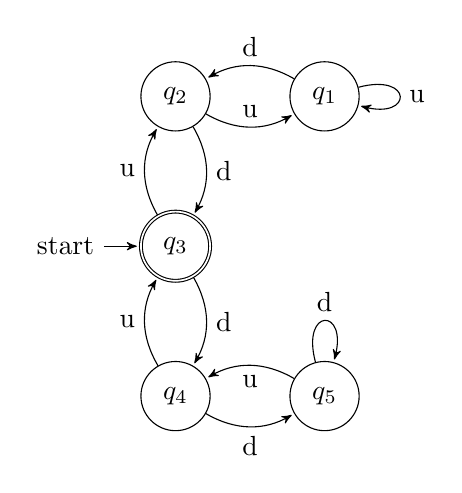
\begin{tikzpicture}[>=stealth',shorten >=1pt,auto,node distance=10mm]

            % define the states in the machine

            \node[initial,state,accepting]  (q3)                    {$q_3$};

            \node[state]                    (q2) [above=of q3]      {$q_2$};

            \node[state]                    (q1) [right=of q2]      {$q_1$};

            \node[state]                    (q4) [below=of q3]      {$q_4$};

            \node[state]                    (q5) [right=of q4]      {$q_5$};

            

            \path[->]   (q1) edge [loop right] node        {u}     (q1) 

                             edge [bend right] node[above] {d}     (q2)

                        (q2) edge [bend right] node        {u}     (q1)

                             edge [bend left]  node        {d}     (q3)

                        (q3) edge [bend left]  node        {u}     (q2)

                             edge [bend left]  node        {d}     (q4)

                        (q4) edge [bend left]  node        {u}     (q3)

                             edge [bend right] node[below] {d}     (q5)

                        (q5) edge [bend right] node        {u}     (q4)

                             edge [loop above] node        {d}     (q5);

        \end{tikzpicture}

    \item [1.4)]

        \begin{itemize}

            \item [a.] $\{\omega | \omega$ has at least three a's$\}$ \\

            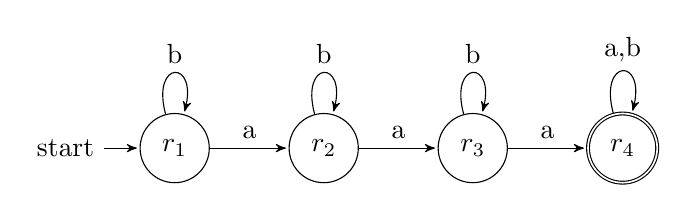
\begin{tikzpicture}[>=stealth',shorten >=1pt,auto,node distance=10mm]

                \node[initial,state] (r1) {$r_1$};

                \node[state] (r2) [right=of r1] {$r_2$};

                \node[state] (r3) [right=of r2] {$r_3$};

                \node[state,accepting] (r4) [right=of r3] {$r_4$};

                

                \foreach \from/\to in {r1/r2, r2/r3, r3/r4}
                    {
                    \path[->] (\from) edge node[above] {a} (\to);
                    }
                    

                \foreach \from in {r1, r2, r3}
                    {
                    \path[->] (\from) edge [loop above] node {b} (\to);
                    }
                    

                \path[->] (r4) edge [loop above] node {a,b} (r4);

            \end{tikzpicture} \\

            $\{\omega | \omega$ has at least two b's$\}$ \\

            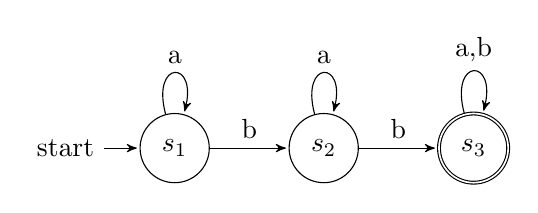
\begin{tikzpicture}[>=stealth',shorten >=1pt,auto,node distance=10mm]

                \node[initial,state] (s1) {$s_1$};

                \node[state] (s2) [right=of s1] {$s_2$};

                \node[state,accepting] (s3) [right=of s2] {$s_3$};

                

                \path[->] (s1) edge node[above] {b} (s2);

                \path[->] (s2) edge node[above] {b} (s3);

                \path[->] (s1) edge [loop above] node {a} (s1);

                \path[->] (s2) edge [loop above] node {a} (s2);

                \path[->] (s3) edge [loop above] node[above] {a,b} (s3);

            \end{tikzpicture} 

            $\{\omega | \omega$ has at least three a's and at least two b's$\}$ \\


            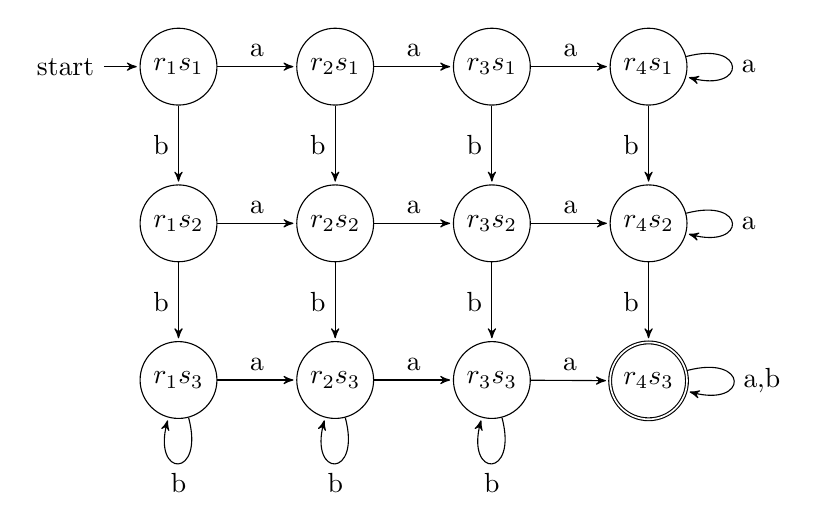
\begin{tikzpicture}[>=stealth',shorten >=1pt,auto,node distance=10mm]

                \node[initial,state] (r1s1) {$r_1s_1$};

                \node[state] (r2s1) [right=of r1s1] {$r_2s_1$};

                \node[state] (r3s1) [right=of r2s1] {$r_3s_1$};

                \node[state] (r4s1) [right=of r3s1] {$r_4s_1$};

                

                \node[state] (r1s2) [below=of r1s1] {$r_1s_2$};

                \node[state] (r2s2) [below=of r2s1] {$r_2s_2$};

                \node[state] (r3s2) [below=of r3s1] {$r_3s_2$};

                \node[state] (r4s2) [below=of r4s1] {$r_4s_2$};

                

                \node[state] (r1s3) [below=of r1s2] {$r_1s_3$};

                \node[state] (r2s3) [below=of r2s2] {$r_2s_3$};

                \node[state] (r3s3) [below=of r3s2] {$r_3s_3$};

                \node[state,accepting] (r4s3) [below=of r4s2] {$r_4s_3$};

                

                \foreach \from/\to in {r1s1/r1s2, r1s2/r1s3, r2s1/r2s2, r2s2/r2s3, r3s1/r3s2, r3s2/r3s3, r4s1/r4s2, r4s2/r4s3}
                    {
                    \path[->] (\from) edge node[left] {b} (\to);
                    }
                    

                \foreach \from/\to in {r1s1/r2s1, r2s1/r3s1, r3s1/r4s1, r1s2/r2s2, r2s2/r3s2, r3s2/r4s2, r1s3/r2s3, r2s3/r3s3, r3s3/r4s3}
                    {
                    \path[->] (\from) edge node[above] {a} (\to);
                    }
                    

                \foreach \from in {r1s3, r2s3, r3s3}
                    {
                    \path[->] (\from) edge [loop below] node[below] {b} (\from);
                    }
                    

                \path[->] (r4s1) edge [loop right] node[right] {a} (r4s1);

                \path[->] (r4s2) edge [loop right] node[right] {a} (r4s2);

                \path[->] (r4s3) edge [loop right] node[right] {a,b} (r4s3);

            \end{tikzpicture}

            \item [c.] $\{\omega | \omega$ has an even number of a's$\}$ \\

            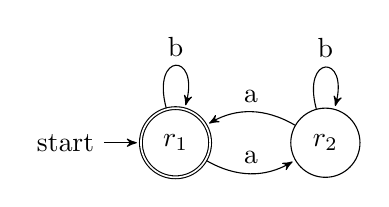
\begin{tikzpicture}[>=stealth',shorten >=1pt,auto,node distance=10mm]

                \node[initial,state,accepting] (r1) {$r_1$};

                \node[state] (r2) [right=of r1] {$r_2$};

                

                \path[->] (r1) edge [bend right] node[above] {a} (r2);

                \path[->] (r2) edge [bend right] node[above] {a} (r1);

                \path[->] (r1) edge [loop above] node {b} (r1);

                \path[->] (r2) edge [loop above] node {b} (r2);

            \end{tikzpicture} \\

            $\{\omega | \omega$ has one or two b's$\}$ \\

            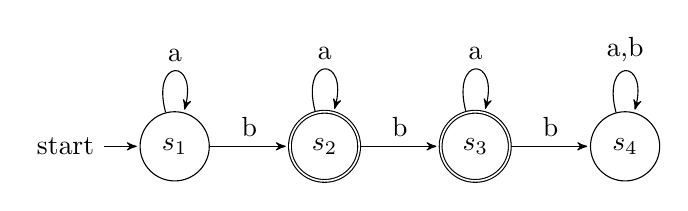
\begin{tikzpicture}[>=stealth',shorten >=1pt,auto,node distance=10mm]

                \node[initial,state] (s1) {$s_1$};

                \node[state,accepting] (s2) [right=of s1] {$s_2$};

                \node[state,accepting] (s3) [right=of s2] {$s_3$};

                \node[state] (s4) [right=of s3] {$s_4$};

                

                \foreach \from/\to in {s1/s2, s2/s3, s3/s4}
                    {
                    \path[->] (\from) edge node[above] {b} (\to);
                    }
                    

                \foreach \from in {s1, s2, s3}
                    {
                    \path[->] (\from) edge [loop above] node {a} (\from);
                    }
                    

                \path[->] (s4) edge [loop above] node {a,b} (s4);

            \end{tikzpicture} \\

            $\{\omega | \omega$ has an even number of a's and one or two b's$\}$ \\

            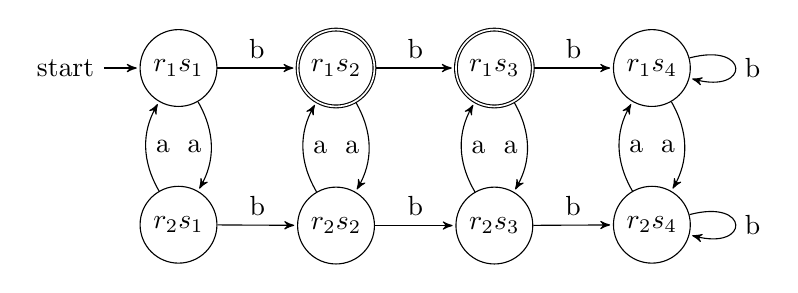
\begin{tikzpicture}[>=stealth',shorten >=1pt,auto,node distance=10mm]

                \node[initial,state] (r1s1) {$r_1s_1$};

                \node[state,accepting] (r1s2) [right=of r1s1] {$r_1s_2$};

                \node[state,accepting] (r1s3) [right=of r1s2] {$r_1s_3$};

                \node[state] (r1s4) [right=of r1s3] {$r_1s_4$};

                

                \node[state] (r2s1) [below=of r1s1] {$r_2s_1$};

                \node[state] (r2s2) [below=of r1s2] {$r_2s_2$};

                \node[state] (r2s3) [below=of r1s3] {$r_2s_3$};

                \node[state] (r2s4) [below=of r1s4] {$r_2s_4$};

                

                \foreach \from/\to in {r1s1/r1s2, r1s2/r1s3, r1s3/r1s4, r2s1/r2s2, r2s2/r2s3, r2s3/r2s4}
                    {
                    \path[->] (\from) edge node[above] {b} (\to);
                    }
                

                \path[->] (r1s4) edge [loop right] node {b} (r1s4);

                \path[->] (r2s4) edge [loop right] node {b} (r2s4);

                

                \foreach \from/\to in {r1s1/r2s1, r1s2/r2s2, r1s3/r2s3, r1s4/r2s4} {

                    \path[->] (\from) edge [bend left] node[left] {a} (\to);

                    \path[->] (\to) edge [bend left] node[right] {a} (\from);

                }

            \end{tikzpicture}

            \item [e.] $\{\omega | \omega$ starts with an a$\}$ \\

            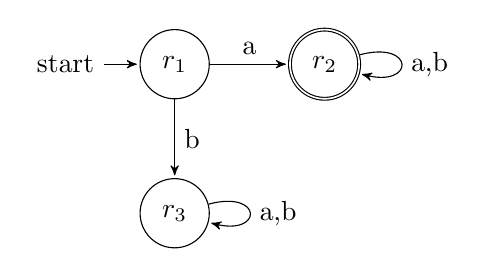
\begin{tikzpicture}[>=stealth',shorten >=1pt,auto,node distance=10mm]

                \node[initial,state] (r1) {$r_1$};

                \node[state,accepting] (r2) [right=of r1] {$r_2$};

                \node[state] (r3) [below=of r1] {$r_3$};

                

                \path[->] (r1) edge node {a} (r2)

                               edge node {b} (r3)

                          (r2) edge [loop right] node {a,b} (r2)

                          (r3) edge [loop right] node {a,b} (r3);

            \end{tikzpicture}

            $\{\omega | \omega$ has at most one b$\}$ \\

            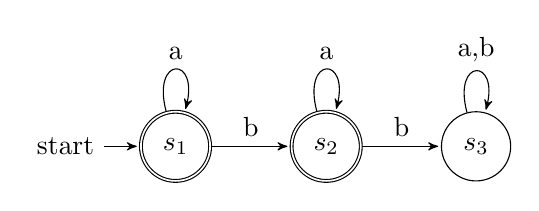
\begin{tikzpicture}[>=stealth',shorten >=1pt,auto,node distance=10mm]

                \node[initial,state,accepting] (s1) {$s_1$};

                \node[state,accepting] (s2) [right=of s1] {$s_2$};

                \node[state] (s3) [right=of s2] {$s_3$};

                

                \path[->] (s1) edge [loop above] node {a} (s1)

                               edge node {b} (s2)

                          (s2) edge [loop above] node {a} (s2)

                               edge node {b} (s3)

                          (s3) edge [loop above] node {a,b} (s3);

            \end{tikzpicture} \\

            $\{\omega | \omega$ starts with an a and has at most one b$\}$ \\

            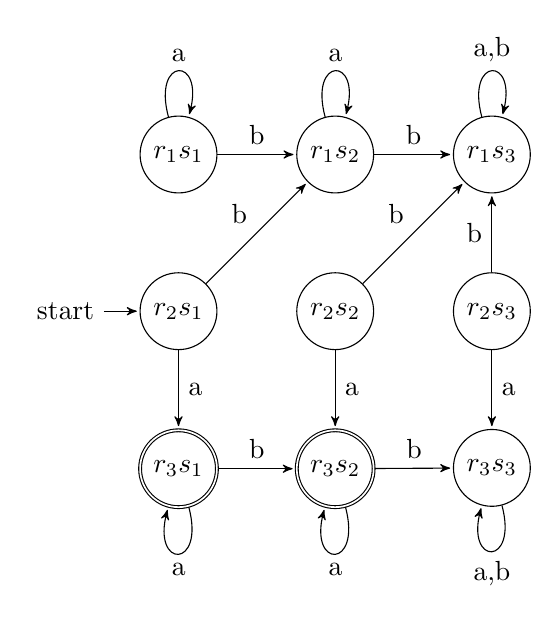
\begin{tikzpicture}[>=stealth',shorten >=1pt,auto,node distance=10mm]

                \node[state] (r1s1) {$r_1s_1$};

                \node[state] (r1s2) [right=of r1s1] {$r_1s_2$};

                \node[state] (r1s3) [right=of r1s2] {$r_1s_3$};

                

                \node[initial,state] (r2s1) [below=of r1s1] {$r_2s_1$};

                \node[state] (r2s2) [below=of r1s2] {$r_2s_2$};

                \node[state] (r2s3) [below=of r1s3] {$r_2s_3$};

                

                \node[state,accepting] (r3s1) [below=of r2s1] {$r_3s_1$};

                \node[state,accepting] (r3s2) [below=of r2s2] {$r_3s_2$};

                \node[state] (r3s3) [below=of r2s3] {$r_3s_3$};

                

                \foreach \from/\to in {r1s1/r1s2, r1s2/r1s3, r3s1/r3s2, r3s2/r3s3, r2s1/r1s2, r2s2/r1s3, r2s3/r1s3}
                    {
                    \path[->] (\from) edge node {b} (\to);
                    }
                    

                \foreach \from/\to in {r2s1/r3s1, r2s2/r3s2, r2s3/r3s3}
                    {
                    \path[->] (\from) edge node {a} (\to);
                    }
                    

                \path[->] (r1s1) edge [loop above] node {a} (r1s1)

                          (r1s2) edge [loop above] node {a} (r1s2)

                          (r1s3) edge [loop above] node {a,b} (r1s3)

                          (r3s1) edge [loop below] node {a} (r3s1)

                          (r3s2) edge [loop below] node {a} (r3s2)

                          (r3s3) edge [loop below] node {a,b} (r3s3);

            \end{tikzpicture}

            \item [f.] $\{\omega | \omega$ has an odd number of a's$\}$ \\

            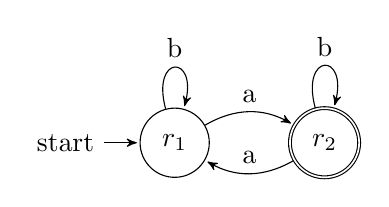
\begin{tikzpicture}[>=stealth',shorten >=1pt,auto,node distance=10mm]

                \node[initial,state] (r1) {$r_1$};

                \node[state,accepting] (r2) [right=of r1] {$r_2$};

                

                \path[->] (r1) edge [bend left] node[above] {a} (r2)

                               edge [loop above] node {b} (r1)

                          (r2) edge [bend left] node[above] {a} (r1)

                               edge [loop above] node {b} (r2);

            \end{tikzpicture} \\

            $\{\omega | \omega$ ends with a b$\}$ \\

            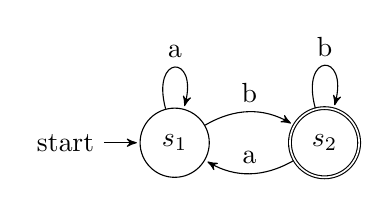
\begin{tikzpicture}[>=stealth',shorten >=1pt,auto,node distance=10mm]

                \node[initial,state] (s1) {$s_1$};

                \node[state,accepting] (s2) [right=of s1] {$s_2$};

                

                \path[->] (s1) edge [bend left] node[above] {b} (s2)

                               edge [loop above] node {a} (s1)

                          (s2) edge [bend left] node[above] {a} (s1)

                               edge [loop above] node {b} (s2);

            \end{tikzpicture} \\

            $\{\omega | \omega$ has an odd number of a's and ends with a b$\}$ \\

            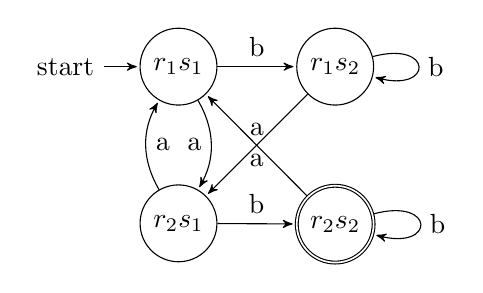
\begin{tikzpicture}[>=stealth',shorten >=1pt,auto,node distance=10mm]

                \node[initial,state] (r1s1) {$r_1s_1$};

                \node[state] (r1s2) [right=of r1s1] {$r_1s_2$};

                \node[state] (r2s1) [below=of r1s1] {$r_2s_1$};

                \node[state,accepting] (r2s2) [below=of r1s2] {$r_2s_2$};

                

                \path[->] (r1s1) edge [bend left] node[left] {a} (r2s1)

                                 edge node {b} (r1s2)

                          (r2s1) edge [bend left] node[right] {a} (r1s1)

                                 edge node {b} (r2s2)

                          (r1s2) edge node[above] {a} (r2s1)

                                 edge [loop right] node {b} (r1s2)

                          (r2s2) edge node[below] {a} (r1s1)

                                 edge [loop right] node {b} (r2s2);

            \end{tikzpicture}


            \item [g.] $\{\omega | \omega$ has an even length$\}$ \\

            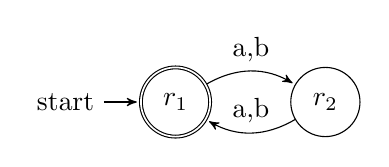
\begin{tikzpicture}[>=stealth',shorten >=1pt,auto,node distance=10mm]

                \node[initial,state,accepting] (r1) {$r_1$};

                \node[state] (r2) [right=of r1] {$r_2$};

                

                \path[->] (r1) edge [bend left] node[above] {a,b} (r2)

                          (r2) edge [bend left] node[above] {a,b} (r1);

            \end{tikzpicture} \\

            $\{\omega | \omega$ has an odd number of a's$\}$ \\

            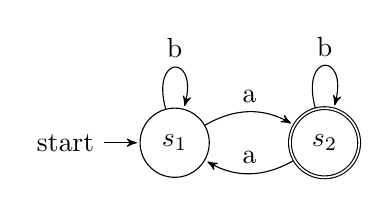
\begin{tikzpicture}[>=stealth',shorten >=1pt,auto,node distance=10mm]

                \node[initial,state] (s1) {$s_1$};

                \node[state,accepting] (s2) [right=of s1] {$s_2$};

                

                \path[->] (s1) edge [bend left] node[above] {a} (s2)

                               edge [loop above] node {b} (s1)

                          (s2) edge [bend left] node[above] {a} (s1)

                               edge [loop above] node {b} (s2);

            \end{tikzpicture} \\

            $\{\omega | \omega$ has an even length and an odd number of a's$\}$ \\

            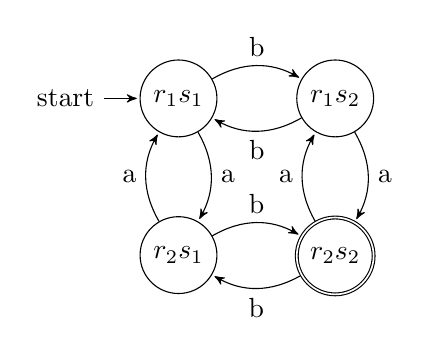
\begin{tikzpicture}[>=stealth',shorten >=1pt,auto,node distance=10mm]

                \node[initial,state] (r1s1) {$r_1s_1$};

                \node[state] (r1s2) [right=of r1s1] {$r_1s_2$};

                \node[state] (r2s1) [below=of r1s1] {$r_2s_1$};

                \node[state,accepting] (r2s2) [below=of r1s2] {$r_2s_2$};

                

                \foreach \from/\to in {r1s1/r2s1, r1s2/r2s2} {

                    \path[->] (\from) edge [bend left] node {a} (\to)

                              (\to) edge [bend left] node {a} (\from);

                }

                

                \foreach \from/\to in {r1s1/r1s2, r2s1/r2s2} {

                    \path[->] (\from) edge [bend left] node {b} (\to)

                              (\to) edge [bend left] node {b} (\from);

                }

            \end{tikzpicture}

        \end{itemize} 

    \item [1.5)]

        \begin{itemize}

            \item [c.] $\{\omega | \omega$ contains the string "ab"$\}$ \\

            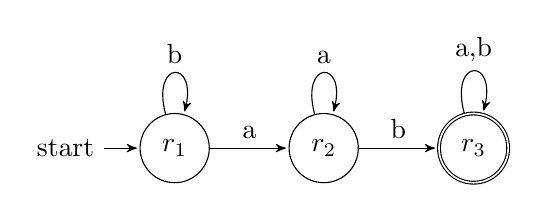
\begin{tikzpicture}[>=stealth',shorten >=1pt,auto,node distance=10mm]

                \node[initial,state] (r1) {$r_1$};

                \node[state] (r2) [right=of r1] {$r_2$};

                \node[state,accepting] (r3) [right=of r2] {$r_3$};

                

                \path[->] (r1) edge node {a} (r2)

                               edge [loop above] node {b} (r1)

                          (r2) edge node {b} (r3)

                               edge [loop above] node {a} (r2)

                          (r3) edge [loop above] node {a,b} (r3);

            \end{tikzpicture} \\

            $\{\omega | \omega$ contains the string "ba"$\}$ \\

            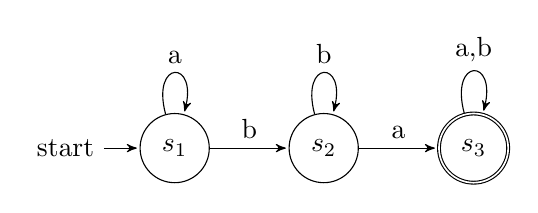
\begin{tikzpicture}[>=stealth',shorten >=1pt,auto,node distance=10mm]

                \node[initial,state] (s1) {$s_1$};

                \node[state] (s2) [right=of s1] {$s_2$};

                \node[state,accepting] (s3) [right=of s2] {$s_3$};

                

                \path[->] (s1) edge node {b} (s2)

                               edge [loop above] node {a} (s1)

                          (s2) edge node {a} (s3)

                               edge [loop above] node {b} (s2)

                          (s3) edge [loop above] node {a,b} (s3);

            \end{tikzpicture} \\

            $\{\omega | \omega$ contains the string "ab" or "ba"$\}$ \\

            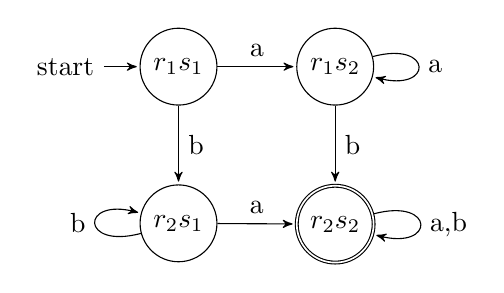
\begin{tikzpicture}[>=stealth',shorten >=1pt,auto,node distance=10mm]

                \node[initial,state] (r1s1) {$r_1s_1$};

                \node[state] (r1s2) [right=of r1s1] {$r_1s_2$};

                \node[state] (r2s1) [below=of r1s1] {$r_2s_1$};

                \node[state,accepting] (r2s2) [below=of r1s2] {$r_2s_2$};

                

                \path[->] (r1s1) edge node {a} (r1s2)

                                 edge node {b} (r2s1)

                          (r1s2) edge [loop right] node {a} (r1s2)

                                 edge node {b} (r2s2)

                          (r2s1) edge [loop left] node {b} (r2s1)

                                 edge node {a} (r2s2)

                          (r2s2) edge [loop right] node {a,b} (r2s2);

            \end{tikzpicture}

            $\{\omega | \omega$ contains neither the string "ab" nor "ba"$\}$ \\

            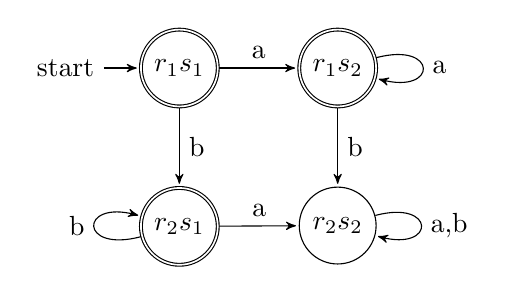
\begin{tikzpicture}[>=stealth',shorten >=1pt,auto,node distance=10mm]

                \node[initial,state,accepting] (r1s1) {$r_1s_1$};

                \node[state,accepting] (r1s2) [right=of r1s1] {$r_1s_2$};

                \node[state,accepting] (r2s1) [below=of r1s1] {$r_2s_1$};

                \node[state] (r2s2) [below=of r1s2] {$r_2s_2$};

                

                \path[->] (r1s1) edge node {a} (r1s2)

                                 edge node {b} (r2s1)

                          (r1s2) edge [loop right] node {a} (r1s2)

                                 edge node {b} (r2s2)

                          (r2s1) edge [loop left] node {b} (r2s1)

                                 edge node {a} (r2s2)

                          (r2s2) edge [loop right] node {a,b} (r2s2);

            \end{tikzpicture}  \newpage

            \item [d.] $\{\omega | \omega$ is any string in $a^*b^*\}$ \\

            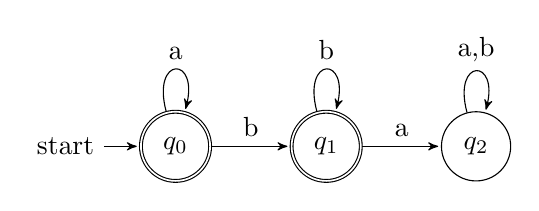
\begin{tikzpicture}[>=stealth',shorten >=1pt,auto,node distance=10mm]

                \node[initial,state,accepting] (q0) {$q_0$};

                \node[state,accepting] (q1) [right=of q0] {$q_1$};

                \node[state] (q2) [right=of q1] {$q_2$};

                

                \path[->] (q0) edge [loop above] node {a} (q0)

                               edge node {b} (q1)

                          (q1) edge [loop above] node {b} (q1)

                               edge node {a} (q2)

                          (q2) edge [loop above] node {a,b} (q2);

            \end{tikzpicture} \\

            $\{\omega | \omega$ is any string not in $a^*b^*\}$ \\

            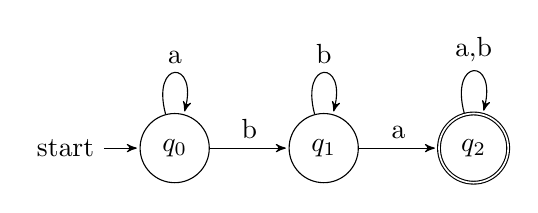
\begin{tikzpicture}[>=stealth',shorten >=1pt,auto,node distance=10mm]

                \node[initial,state] (q0) {$q_0$};

                \node[state] (q1) [right=of q0] {$q_1$};

                \node[state,accepting] (q2) [right=of q1] {$q_2$};

                

                \path[->] (q0) edge [loop above] node {a} (q0)

                               edge node {b} (q1)

                          (q1) edge [loop above] node {b} (q1)

                               edge node {a} (q2)

                          (q2) edge [loop above] node {a,b} (q2);

            \end{tikzpicture}

            \item [e.] $\{\omega | \omega$ is any string in $(ab^*)^*\}$ \\

            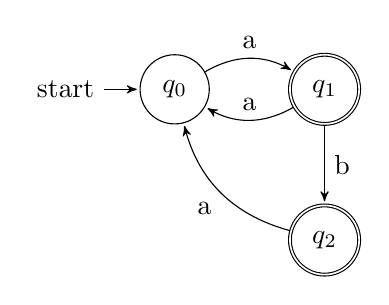
\begin{tikzpicture}[>=stealth',shorten >=1pt,auto,node distance=10mm]

                \node[initial,state] (q0) {$q_0$};

                \node[state,accepting] (q1) [right=of q0] {$q_1$};

                \node[state,accepting] (q2) [below=of q1] {$q_2$};

                

                \path[->] (q0) edge [bend left] node[above] {a} (q1)

                          (q1) edge [bend left] node[above] {a} (q0)

                               edge node {b} (q2)

                          (q2) edge [bend left] node {a} (q0);

            \end{tikzpicture} \\

            $\{\omega | \omega$ is any string not in $(ab^*)^*\}$ \\

            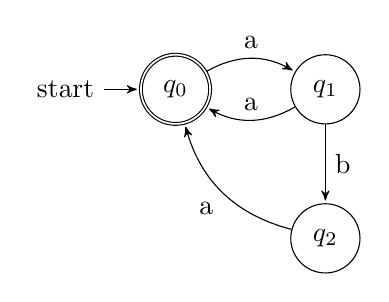
\begin{tikzpicture}[>=stealth',shorten >=1pt,auto,node distance=10mm]

                \node[initial,state,accepting] (q0) {$q_0$};

                \node[state] (q1) [right=of q0] {$q_1$};

                \node[state] (q2) [below=of q1] {$q_2$};

                

                \path[->] (q0) edge [bend left] node[above] {a} (q1)

                          (q1) edge [bend left] node[above] {a} (q0)

                               edge node {b} (q2)

                          (q2) edge [bend left] node {a} (q0);

            \end{tikzpicture} 

            \item [f.] $\{\omega | \omega$ is any string in a* $\cup$ b*$\}$ \\

            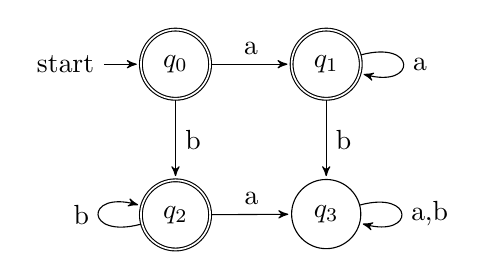
\begin{tikzpicture}[>=stealth',shorten >=1pt,auto,node distance=10mm]

                \node[initial,state,accepting] (q0) {$q_0$};

                \node[state,accepting] (q1) [right=of q0] {$q_1$};

                \node[state,accepting] (q2) [below=of q0] {$q_2$};

                \node[state] (q3) [below=of q1] {$q_3$};

                

                \path[->] (q0) edge node {a} (q1)

                               edge node {b} (q2)

                          (q1) edge [loop right] node {a} (q1)

                               edge node {b} (q3)

                          (q2) edge [loop left] node {b} (q2)

                               edge node {a} (q3)

                          (q3) edge [loop right] node {a,b} (q3);

            \end{tikzpicture} \\

            $\{\omega | \omega$ is any string not in a* $\cup$ b*$\}$ \\

            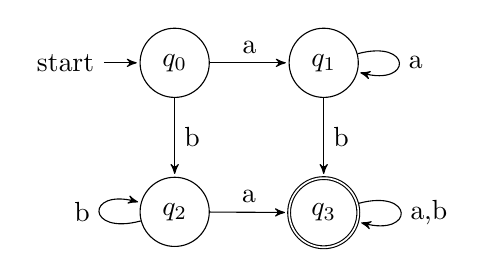
\begin{tikzpicture}[>=stealth',shorten >=1pt,auto,node distance=10mm]

                \node[initial,state] (q0) {$q_0$};

                \node[state] (q1) [right=of q0] {$q_1$};

                \node[state] (q2) [below=of q0] {$q_2$};

                \node[state,accepting] (q3) [below=of q1] {$q_3$};

                

                \path[->] (q0) edge node {a} (q1)

                               edge node {b} (q2)

                          (q1) edge [loop right] node {a} (q1)

                               edge node {b} (q3)

                          (q2) edge [loop left] node {b} (q2)

                               edge node {a} (q3)

                          (q3) edge [loop right] node {a,b} (q3);

            \end{tikzpicture} \newpage

            \item [g.] $\{\omega | \omega$ is any string that contains exactly two a's$\}$ \\

            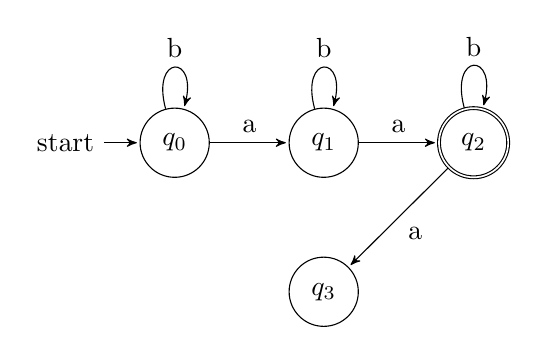
\begin{tikzpicture}[>=stealth',shorten >=1pt,auto,node distance=10mm]

                \node[initial,state] (q0) {$q_0$};

                \node[state] (q1) [right=of q0] {$q_1$};

                \node[state,accepting] (q2) [right=of q1] {$q_2$};

                \node[state] (q3) [below=of q1] {$q_3$};

                

                \path[->] (q0) edge [loop above] node {b} (q0)

                               edge node {a} (q1)

                          (q1) edge [loop above] node {b} (q1)

                               edge node {a} (q2)

                          (q2) edge [loop above] node {b} (q2)

                               edge node {a} (q3);

            \end{tikzpicture} \\

            $\{\omega | \omega$ is any string that doesn't contain exactly two a's$\}$ \\

            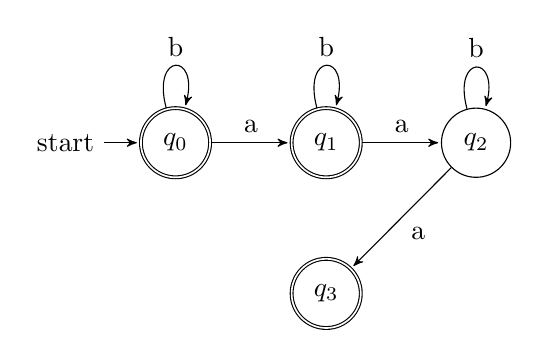
\begin{tikzpicture}[>=stealth',shorten >=1pt,auto,node distance=10mm]

                \node[initial,state,accepting] (q0) {$q_0$};

                \node[state,accepting] (q1) [right=of q0] {$q_1$};

                \node[state] (q2) [right=of q1] {$q_2$};

                \node[state,accepting] (q3) [below=of q1] {$q_3$};

                

                \path[->] (q0) edge [loop above] node {b} (q0)

                               edge node {a} (q1)

                          (q1) edge [loop above] node {b} (q1)

                               edge node {a} (q2)

                          (q2) edge [loop above] node {b} (q2)

                               edge node {a} (q3);

            \end{tikzpicture} 

            \item [h.] $\{\omega | \omega$ is the string "a" or the string "b"$\}$ \\

            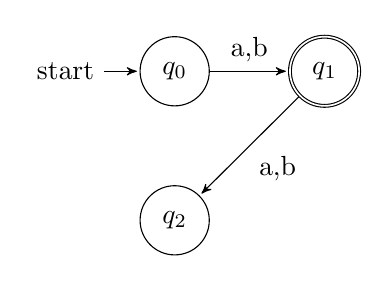
\begin{tikzpicture}[>=stealth',shorten >=1pt,auto,node distance=10mm]

                \node[initial,state] (q0) {$q_0$};

                \node[state,accepting] (q1) [right=of q0] {$q_1$};

                \node[state] (q2) [below=of q0] {$q_2$};

                

                \path[->] (q0) edge node[above] {a,b} (q1)

                          (q1) edge node {a,b} (q2);

            \end{tikzpicture} \\

            $\{\omega | \omega$ is any string except "a" and "b"$\}$ \\

            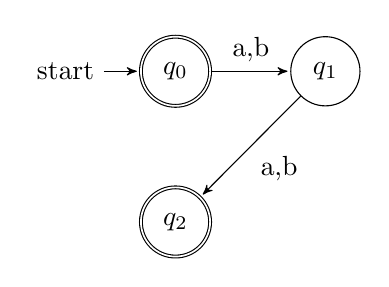
\begin{tikzpicture}[>=stealth',shorten >=1pt,auto,node distance=10mm]

                \node[initial,state,accepting] (q0) {$q_0$};

                \node[state] (q1) [right=of q0] {$q_1$};

                \node[state,accepting] (q2) [below=of q0] {$q_2$};

                

                \path[->] (q0) edge node[above] {a,b} (q1)

                          (q1) edge node {a,b} (q2);

            \end{tikzpicture}

        \end{itemize}

    \item [1.6)]

    \begin{itemize}

        \item [a.] $\{\omega | \omega$ begins with a 1 and ends with a 0$\}$ \\

        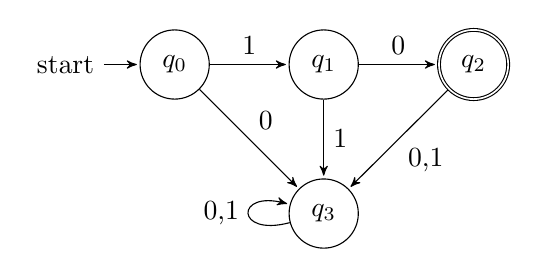
\begin{tikzpicture}[>=stealth',shorten >=1pt,auto,node distance=10mm]

            \node[initial,state] (q0) {$q_0$};

            \node[state] (q1) [right=of q0] {$q_1$};

            \node[state,accepting] (q2) [right=of q1] {$q_2$};

            \node[state] (q3) [below=of q1] {$q_3$};

            

            \path[->] (q0) edge node {1} (q1)

                           edge node {0} (q3)

                      (q1) edge node {0} (q2)

                           edge node {1} (q3)

                      (q2) edge node {0,1} (q3)

                      (q3) edge [loop left] node {0,1} (q3);

        \end{tikzpicture} \newpage

        \item [b.] $\{\omega | \omega$ contains at least three 1's$\}$ \\

        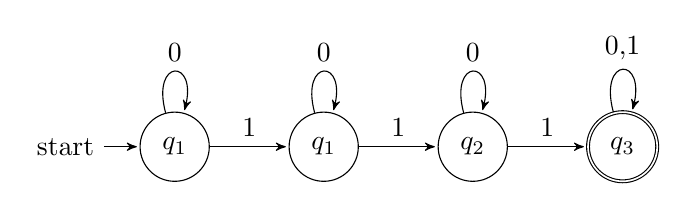
\begin{tikzpicture}[>=stealth',shorten >=1pt,auto,node distance=10mm]

            \node[initial,state] (q0) {$q_1$};

            \node[state] (q1) [right=of q0] {$q_1$};

            \node[state] (q2) [right=of q1] {$q_2$};

            \node[state,accepting] (q3) [right=of q2] {$q_3$};

            

            \path[->] (q0) edge [loop above] node {0} (q0)

                           edge node {1} (q1)

                      (q1) edge [loop above] node {0} (q1)

                           edge node {1} (q2)

                      (q2) edge [loop above] node {0} (q2)

                           edge node {1} (q3)

                      (q3) edge [loop above] node {0,1} (q3);

            \end{tikzpicture} 

        \item [c.] $\{\omega | \omega$ contains the substring 0101$\}$ \\

        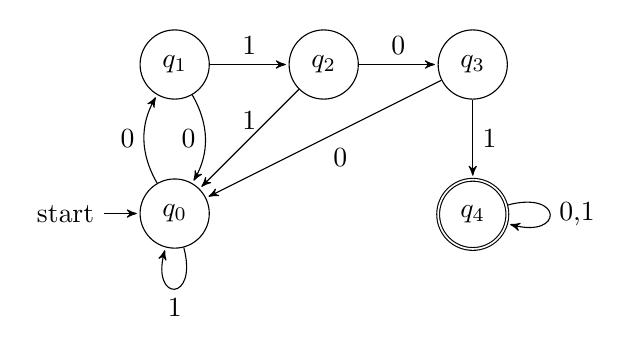
\begin{tikzpicture}[>=stealth',shorten >=1pt,auto,node distance=10mm]

            \node[initial,state] (q0) {$q_0$};

            \node[state] (q1) [above=of q0] {$q_1$};

            \node[state] (q2) [right=of q1] {$q_2$};

            \node[state] (q3) [right=of q2] {$q_3$};

            \node[state,accepting] (q4) [below=of q3] {$q_4$};

            

            \path[->] (q0) edge [bend left] node[left] {0} (q1)

                           edge [loop below] node {1} (q0)

                      (q1) edge [bend left] node[left] {0} (q0)

                           edge node {1} (q2)

                      (q2) edge node[above] {1} (q0)

                           edge node {0} (q3)

                      (q3) edge node {0} (q0)

                           edge node {1} (q4)

                      (q4) edge [loop right] node {0,1} (q4);

        \end{tikzpicture} 

        \item [d.] $\{\omega | \omega$ has a length at least 3 and the third symbol is a 0$\}$ \\

        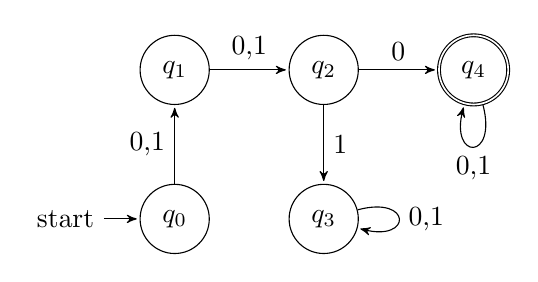
\begin{tikzpicture}[>=stealth',shorten >=1pt,auto,node distance=10mm]

            \node[initial,state] (q0) {$q_0$};

            \node[state] (q1) [above=of q0] {$q_1$};

            \node[state] (q2) [right=of q1] {$q_2$};

            \node[state] (q3) [below=of q2] {$q_3$};

            \node[state,accepting] (q4) [right=of q2] {$q_4$};

            

            \path[->] (q0) edge node {0,1} (q1)

                      (q1) edge node {0,1} (q2)

                      (q2) edge node {0} (q4)

                           edge node {1} (q3)

                      (q3) edge [loop right] node {0,1} (q3)

                      (q4) edge [loop below] node {0,1} (q4);

        \end{tikzpicture}

        \item [e.] $\{\omega | \omega$ starts with a 0 and has an odd length or starts with a 1 and has an even length$\}$ \\

        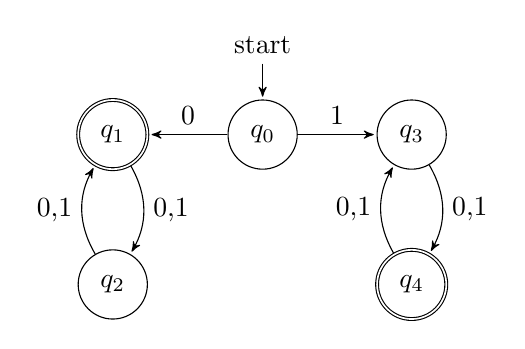
\begin{tikzpicture}[>=stealth',shorten >=1pt,auto,node distance=10mm]

            \node[initial,state,initial where=above] (q0) {$q_0$};

            \node[state,accepting] (q1) [left=of q0] {$q_1$};

            \node[state] (q3) [right=of q0] {$q_3$};

            \node[state] (q2) [below=of q1] {$q_2$};

            \node[state,accepting] (q4) [below=of q3] {$q_4$};

            

            \path[->] (q0) edge node[above] {0} (q1)

                           edge node[above] {1} (q3)

                      (q1) edge [bend left] node[right] {0,1} (q2)

                      (q2) edge [bend left] node[left] {0,1} (q1)

                      (q3) edge [bend left] node[right] {0,1} (q4)

                      (q4) edge [bend left] node[left] {0,1} (q3);

        \end{tikzpicture} 

        \item [f.] $\{\omega | \omega$ contains the substring 110$\}$ \\

        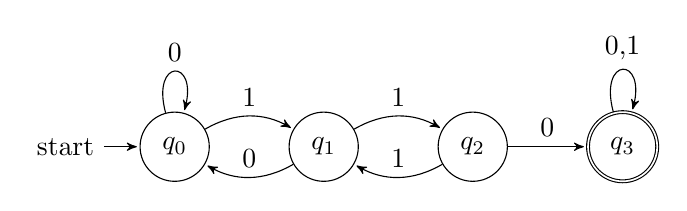
\begin{tikzpicture}[>=stealth',shorten >=1pt,auto,node distance=10mm]

            \node[initial,state] (q0) {$q_0$};

            \node[state] (q1) [right=of q0] {$q_1$};

            \node[state] (q2) [right=of q1] {$q_2$};

            \node[state,accepting] (q3) [right=of q2] {$q_3$};

            

            \path[->] (q0) edge [loop above] node {0} (q0)

                           edge [bend left] node[above] {1} (q1)

                      (q1) edge [bend left] node[above] {0} (q0)

                           edge [bend left] node[above] {1} (q2)

                      (q2) edge node {0} (q3)

                           edge [bend left] node[above] {1} (q1)

                      (q3) edge [loop above] node {0,1} (q3);

        \end{tikzpicture} \newpage

        $\{\omega | \omega$ does not contain the substring 110$\}$ \\

        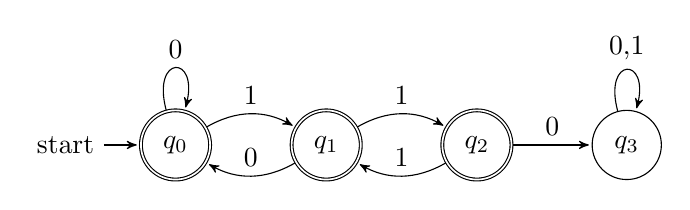
\begin{tikzpicture}[>=stealth',shorten >=1pt,auto,node distance=10mm]

            \node[initial,state,accepting] (q0) {$q_0$};

            \node[state,accepting] (q1) [right=of q0] {$q_1$};

            \node[state,accepting] (q2) [right=of q1] {$q_2$};

            \node[state] (q3) [right=of q2] {$q_3$};

            

            \path[->] (q0) edge [loop above] node {0} (q0)

                           edge [bend left] node[above] {1} (q1)

                      (q1) edge [bend left] node[above] {0} (q0)

                           edge [bend left] node[above] {1} (q2)

                      (q2) edge node {0} (q3)

                           edge [bend left] node[above] {1} (q1)

                      (q3) edge [loop above] node {0,1} (q3);

        \end{tikzpicture}

        \item [g.] $\{\omega | \omega$'s length is at most 5$\}$ \\

        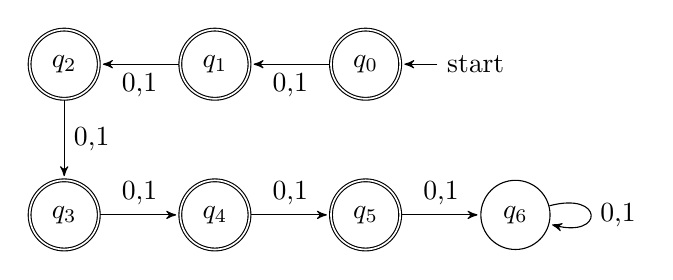
\begin{tikzpicture}[>=stealth',shorten >=1pt,auto,node distance=10mm]

            \node[initial,state,accepting,initial where=right] (q0) {$q_0$};

            \node[state,accepting] (q1) [left=of q0] {$q_1$};

            \node[state,accepting] (q2) [left=of q1] {$q_2$};

            \node[state,accepting] (q3) [below=of q2] {$q_3$};

            \node[state,accepting] (q4) [right=of q3] {$q_4$};

            \node[state,accepting] (q5) [right=of q4] {$q_5$};

            \node[state] (q6) [right=of q5] {$q_6$};

            

            \foreach \from/\to in {q0/q1, q1/q2, q2/q3, q3/q4, q4/q5, q5/q6}
	   {
                \path[->] (\from) edge node {0,1} (\to);
              }
            \path[->] (q6) edge [loop right] node {0,1} (q6);

        \end{tikzpicture} 

        \item [h.] $\{\omega | \omega$ is the string 11 or 111$\}$ \\

        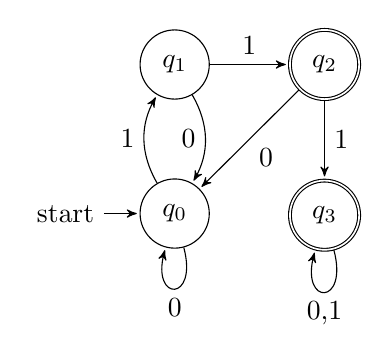
\begin{tikzpicture}[>=stealth',shorten >=1pt,auto,node distance=10mm]

            \node[initial,state] (q0) {$q_0$};

            \node[state] (q1) [above=of q0] {$q_1$};

            \node[state,accepting] (q2) [right=of q1] {$q_2$};

            \node[state,accepting] (q3) [below=of q2] {$q_3$};

            

            \path[->] (q0) edge [loop below] node {0} (q0)

                           edge [bend left] node[left] {1} (q1)

                      (q1) edge [bend left] node[left] {0} (q0)

                           edge node {1} (q2)

                      (q2) edge node {0} (q0)

                           edge node {1} (q3)

                      (q3) edge [loop below] node {0,1} (q3);

        \end{tikzpicture} \\

        $\{\omega | \omega$ is any string except 11 and 111$\}$ \\

        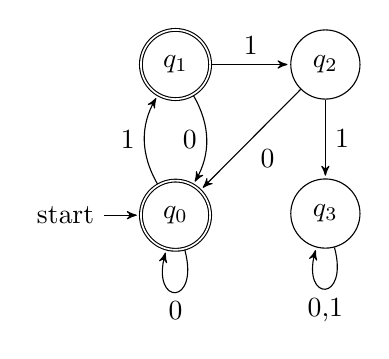
\begin{tikzpicture}[>=stealth',shorten >=1pt,auto,node distance=10mm]

            \node[initial,state,accepting] (q0) {$q_0$};

            \node[state,accepting] (q1) [above=of q0] {$q_1$};

            \node[state] (q2) [right=of q1] {$q_2$};

            \node[state] (q3) [below=of q2] {$q_3$};

            

            \path[->] (q0) edge [loop below] node {0} (q0)

                           edge [bend left] node[left] {1} (q1)

                      (q1) edge [bend left] node[left] {0} (q0)

                           edge node {1} (q2)

                      (q2) edge node {0} (q0)

                           edge node {1} (q3)

                      (q3) edge [loop below] node {0,1} (q3);

        \end{tikzpicture}

        \item [i.] $\{\omega | $every odd position in $\omega$ is a 1$\}$ \\

        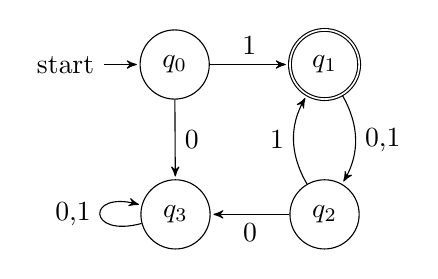
\begin{tikzpicture}[>=stealth',shorten >=1pt,auto,node distance=10mm]

            \node[initial,state] (q0) {$q_0$};

            \node[state,accepting] (q1) [right=of q0] {$q_1$};

            \node[state] (q2) [below=of q1] {$q_2$};

            \node[state] (q3) [left=of q2] {$q_3$};

            

            \path[->] (q0) edge node {1} (q1)

                           edge node {0} (q3)

                      (q1) edge [bend left] node[right] {0,1} (q2)

                      (q2) edge [bend left] node[left] {1} (q1)

                           edge node {0} (q3)

                      (q3) edge [loop left] node {0,1} (q3);

        \end{tikzpicture}

        \item [j.] $\{\omega | \omega$ contains at least two 2's and at most one 1$\}$ \\

        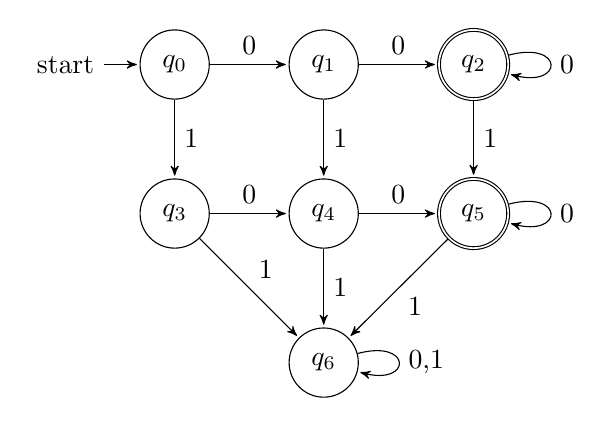
\begin{tikzpicture}[>=stealth',shorten >=1pt,auto,node distance=10mm]

            \node[initial,state] (q0) {$q_0$};

            \node[state] (q1) [right=of q0] {$q_1$};

            \node[state,accepting] (q2) [right=of q1] {$q_2$};

            \node[state] (q3) [below=of q0] {$q_3$};

            \node[state] (q4) [right=of q3] {$q_4$};

            \node[state,accepting] (q5) [right=of q4] {$q_5$};

            \node[state] (q6) [below=of q4] {$q_6$};

            

            \path[->] (q0) edge node {0} (q1)

                           edge node {1} (q3)

                      (q1) edge node {0} (q2)

                           edge node {1} (q4)

                      (q2) edge [loop right] node {0} (q2)

                           edge node {1} (q5)

                      (q3) edge node {0} (q4)

                           edge node {1} (q6)

                      (q4) edge node {0} (q5)

                           edge node {1} (q6)

                      (q5) edge [loop right] node {0} (q5)

                           edge node {1} (q6)

                      (q6) edge [loop right] node {0,1} (q6);

        \end{tikzpicture} 

        \item [k.] $\{\varepsilon, 0\}$ \\

        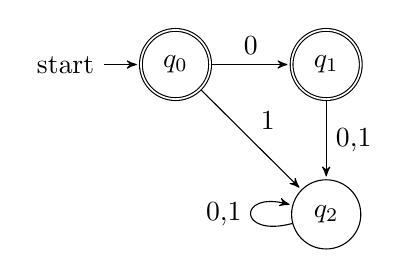
\begin{tikzpicture}[>=stealth',shorten >=1pt,auto,node distance=10mm]

            \node[initial,state,accepting] (q0) {$q_0$};

            \node[state,accepting] (q1) [right=of q0] {$q_1$};

            \node[state] (q2) [below=of q1] {$q_2$};

            

            \path[->] (q0) edge node {0} (q1)

                           edge node {1} (q2)

                      (q1) edge node {0,1} (q2)

                      (q2) edge [loop left] node {0,1} (q2);

        \end{tikzpicture}

        \item [l.] $\{\omega | \omega$ contains an even number of 0's, or contains exactly two 1's$\}$ \\

        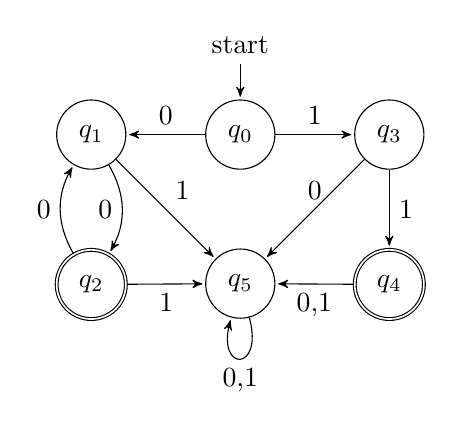
\begin{tikzpicture}[>=stealth',shorten >=1pt,auto,node distance=10mm]

            \node[initial,state,initial where=above] (q0) {$q_0$};

            \node[state] (q1) [left=of q0] {$q_1$};

            \node[state,accepting] (q2) [below=of q1] {$q_2$};

            \node[state] (q3) [right=of q0] {$q_3$};

            \node[state,accepting] (q4) [below=of q3] {$q_4$};

            \node[state] (q5) [below=of q0] {$q_5$};

            

            \path[->] (q0) edge node[above] {0} (q1)

                           edge node {1} (q3)

                      (q1) edge [bend left] node[left] {0} (q2)

                           edge node {1} (q5)

                      (q2) edge [bend left] node[left] {0} (q1)

                           edge node[below] {1} (q5)

                      (q3) edge node {1} (q4)

                           edge node[above] {0} (q5)

                      (q4) edge node {0,1} (q5)

                      (q5) edge [loop below] node {0,1} (q5);

        \end{tikzpicture}

        \item [m.] The empty set \\

        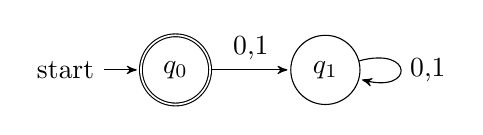
\begin{tikzpicture}[>=stealth',shorten >=1pt,auto,node distance=10mm]

            \node[initial,state,accepting] (q0) {$q_0$};

            \node[state] (q1) [right=of q0] {$q_1$};

            

            \path[->] (q0) edge node {0,1} (q1)

                      (q1) edge [loop right] node {0,1} (q1);

        \end{tikzpicture}

        \item [n.] All strings except the empty string \\

        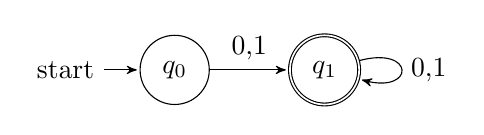
\begin{tikzpicture}[>=stealth',shorten >=1pt,auto,node distance=10mm]

            \node[initial,state] (q0) {$q_0$};

            \node[state,accepting] (q1) [right=of q0] {$q_1$};

            

            \path[->] (q0) edge node {0,1} (q1)

                      (q1) edge [loop right] node {0,1} (q1);

        \end{tikzpicture}

    \end{itemize}

    \item [1.7)]

    \begin{itemize}

        \item [b.] Exercise 1.6c with five states \\

        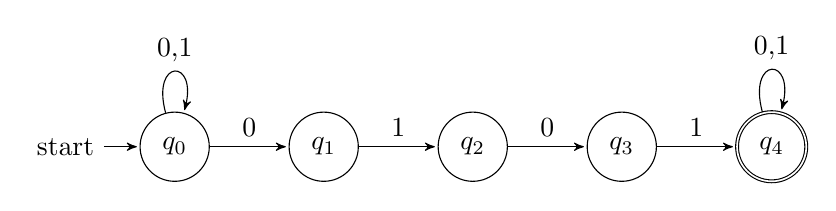
\begin{tikzpicture}[>=stealth',shorten >=1pt,auto,node distance=10mm]

            \node[initial,state] (q0) {$q_0$};

            \node[state] (q1) [right=of q0] {$q_1$};

            \node[state] (q2) [right=of q1] {$q_2$};

            \node[state] (q3) [right=of q2] {$q_3$};

            \node[state,accepting] (q4) [right=of q3] {$q_4$};

            

            \path[->] (q0) edge [loop above] node {0,1} (q0)

                           edge node {0} (q1)

                      (q1) edge node {1} (q2)

                      (q2) edge node {0} (q3)

                      (q3) edge node {1} (q4)

                      (q4) edge [loop above] node {0,1} (q4);

        \end{tikzpicture} 

        \item [c.] Exercise 1.6l with 6 states \\

        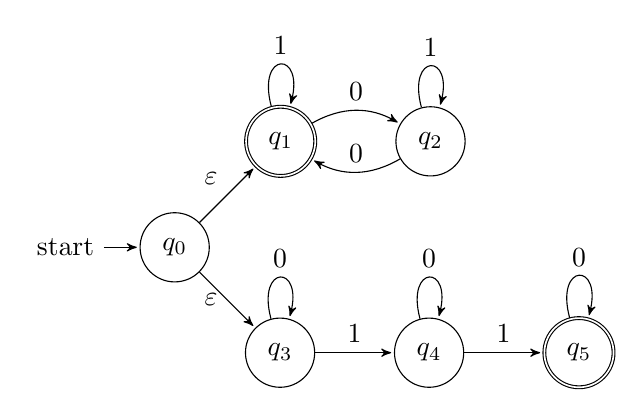
\begin{tikzpicture}[>=stealth',shorten >=1pt,auto,node distance=10mm]

            \node[initial,state] (q0) {$q_0$};

            \node[state,accepting] (q1) [above right=of q0] {$q_1$};

            \node[state] (q2) [right=of q1] {$q_2$};

            \node[state] (q3) [below right=of q0] {$q_3$};

            \node[state] (q4) [right=of q3] {$q_4$};

            \node[state,accepting] (q5) [right=of q4] {$q_5$};

            

            \path[->] (q0) edge node {$\varepsilon$} (q1)

                           edge node[left] {$\varepsilon$} (q3)

                      (q1) edge [bend left] node[above] {0} (q2)

                           edge [loop above] node {1} (q1)

                      (q2) edge [bend left] node[above] {0} (q1)

                           edge [loop above] node {1} (q2)

                      (q3) edge [loop above] node {0} (q3)

                           edge node {1} (q4)

                      (q4) edge [loop above] node {0} (q4)

                           edge node {1} (q5)

                      (q5) edge [loop above] node {0} (q5);

        \end{tikzpicture} 

        \item [d.] The language $\{0\}$ with two states \\

        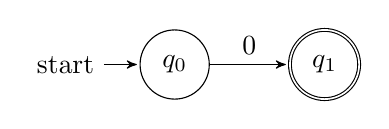
\begin{tikzpicture}[>=stealth',shorten >=1pt,auto,node distance=10mm]

            \node[initial,state] (q0) {$q_0$};

            \node[state,accepting] (q1) [right=of q0] {$q_1$};

            

            \path[->] (q0) edge node {0} (q1);

        \end{tikzpicture}

        \item [e.] The language $0^*1^*0^+$ with three states \\

        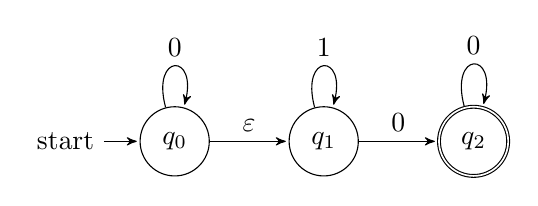
\begin{tikzpicture}[>=stealth',shorten >=1pt,auto,node distance=10mm]

            \node[initial,state] (q0) {$q_0$};

            \node[state] (q1) [right=of q0] {$q_1$};

            \node[state,accepting] (q2) [right=of q1] {$q_2$};

            

            \path[->] (q0) edge [loop above] node {0} (q0)

                           edge node {$\varepsilon$} (q1)

                      (q1) edge [loop above] node {1} (q1)

                           edge node {0} (q2)

                      (q2) edge [loop above] node {0} (q2);

        \end{tikzpicture}

        \item [g.] The language $\varepsilon$ with one state \\

        \begin{tikzpicture}[>=stealth',shorten >=1pt,auto,node distance=10mm]

            \node[initial,state,accepting] (q0) {$q_0$};

        \end{tikzpicture}

        \item [h.] The language $0^*$ with one state \\

        \begin{tikzpicture}[>=stealth',shorten >=1pt,auto,node distance=10mm]

            \node[initial,state,accepting] (q0) {$q_0$};

            \path[->] (q0) edge [loop right] node {0} (q0);

        \end{tikzpicture}

    \end{itemize}

    \item [1.8)]

    \begin{itemize}

        \item [a.] The NFA of the union of the languages in exercises 1.6a and 1.6b \\

        \begin{tikzpicture}[>=stealth',shorten >=1pt,auto,node distance=10mm]

            \node[initial,state] (q0) {$q_0$};

            \node[state] (q1) [above right=of q0] {$q_1$};

            \node[state] (q2) [right=of q1] {$q_2$};

            \node[state,accepting] (q3) [right=of q2] {$q_3$};

            \node[state] (q4) [below right=of q0] {$q_4$};

            \node[state] (q5) [right=of q4] {$q_5$};

            \node[state] (q6) [right=of q5] {$q_6$};

            \node[state,accepting] (q7) [right=of q6] {$q_7$};

            

            \path[->] (q0) edge node {$\varepsilon$} (q1)

                           edge node {$\varepsilon$} (q4)

                      (q1) edge node {1} (q2)

                      (q2) edge [loop above] node {0,1} (q2)

                           edge node {0} (q3)

                      (q4) edge [loop above] node {0} (q4)

                           edge node {1} (q5)

                      (q5) edge [loop above] node {0} (q5)

                           edge node {1} (q6)

                      (q6) edge [loop above] node {0} (q6)

                           edge node {1} (q7)

                      (q7) edge [loop above] node {0,1} (q7);

        \end{tikzpicture} \newpage

        \item [b.] The NFA of the union of the languages in exercises 1.6c and 1.6f \\

        \begin{tikzpicture}[>=stealth',shorten >=1pt,auto,node distance=10mm]

            \node[initial,state] (q0) {$q_0$};

            \node[state] (q1) [above right=of q0] {$q_1$};

            \node[state] (q2) [right=of q1] {$q_2$};

            \node[state] (q3) [right=of q2] {$q_3$};

            \node[state] (q4) [right=of q3] {$q_4$};

            \node[state,accepting] (q5) [right=of q4] {$q_5$};

            \node[state,accepting] (q6) [below right=of q0] {$q_6$};

            \node[state,accepting] (q7) [right=of q6] {$q_7$};

            \node[state,accepting] (q8) [right=of q7] {$q_8$};

            \node[state] (q9) [right=of q8] {$q_9$};

            

            \path[->] (q0) edge node {$\varepsilon$} (q1)

                           edge node[left] {$\varepsilon$} (q6)

                      (q1) edge [loop above] node {0,1} (q1)

                           edge node {0} (q2)

                      (q2) edge node {1} (q3)

                      (q3) edge node {0} (q4)

                      (q4) edge node {1} (q5)

                      (q5) edge [loop above] node {0,1} (q5)

                      (q6) edge [loop above] node {0,1} (q6)

                           edge node {1} (q7)

                      (q7) edge node {1} (q8)

                      (q8) edge node {0} (q9)

                      (q9) edge [loop above] node {0,1} (q9);

        \end{tikzpicture}

    \end{itemize}

    \item [1.9)]

    \begin{itemize}

        \item [a.] The NFA of the concatenation of the languages in exercises 1.6g and 1.6i \\

        \begin{tikzpicture}[>=stealth',shorten >=1pt,auto,node distance=10mm]

            \node[initial,state] (r0) {$r_0$};

            \node[state] (r1) [right=of r0] {$r_1$};

            \node[state] (r2) [right=of r1] {$r_2$};

            \node[state] (r3) [right=of r2] {$r_3$};

            \node[state] (r4) [right=of r3] {$r_4$};

            \node[state] (r5) [right=of r4] {$r_5$};

            \node[state,accepting] (s0) [below=of r3] {$s_0$};

            \node[state,accepting] (s1) [right=of s0] {$s_1$};

            \node[state,accepting] (s2) [right=of s1] {$s_2$};

            \node[state] (s3) [right=of s2] {$s_3$};

            

            \foreach \from/\to in {r0/r1, r1/r2, r2/r3, r3/r4, r4/r5}
	 {
                \path[->] (\from) edge node {0,1} (\to)
                                  edge node {$\varepsilon$} (s0);
	 }
            \path[->] (r5) edge [loop right] node {0,1} (r5)

                      (s0) edge node {1} (s1)

                           edge [bend right] node[below] {0} (s3)

                      (s1) edge [bend left] node[above] {0,1} (s2)

                      (s2) edge [bend left] node[below] {1} (s1)

                           edge node {0} (s3)

                      (s3) edge [loop above] node {0,1} (s3);

        \end{tikzpicture}

        \item [b.] The NFA of the concatenation of the languages in exercises 1.6b and 1.6m \\

        \begin{tikzpicture}[>=stealth',shorten >=1pt,auto,node distance=10mm]

            \node[initial,state] (r0) {$r_0$};

            \node[state] (r1) [right=of r0] {$r_1$};

            \node[state] (r2) [right=of r1] {$r_2$};

            \node[state] (r3) [right=of r2] {$r_3$};

            \node[state,accepting] (s0) [right=of r3] {$s_0$};

            

            \foreach \from/\to in {r0/r1, r1/r2, r2/r3}
	 {
                \path[->] (\from) edge node {1} (\to)

                                  edge [loop above] node {0} (\from);
	 }
            \path[->] (r3) edge [loop above] node {0,1} (r3)

                           edge node {$\varepsilon$} (s0);

        \end{tikzpicture}

    \end{itemize}

    \item [1.10)]

    \begin{itemize}

        \item [a.] The star of the language in exercise 1.6b \\

        \begin{tikzpicture}[>=stealth',shorten >=1pt,auto,node distance=10mm]

            \node[initial,state,accepting] (q0) {$q_1$};

            \node[state] (q1) [right=of q0] {$q_1$};

            \node[state] (q2) [right=of q1] {$q_2$};

            \node[state] (q3) [right=of q2] {$q_3$};

            \node[state,accepting] (q4) [right=of q3] {$q_4$};

            

            \path[->] (q0) edge node {$\varepsilon$} (q1)

                      (q1) edge [loop above] node {0} (q1)

                           edge node {1} (q2)

                      (q2) edge [loop above] node {0} (q2)

                           edge node {1} (q3)

                      (q3) edge [loop above] node {0} (q3)

                           edge node {1} (q4)

                      (q4) edge [loop above] node {0,1} (q4)

                           edge [bend left] node {$\varepsilon$} (q0);

        \end{tikzpicture} \newpage

        \item [b.] The star of exercise 1.6j (I couldn't figure out a way to make this graph look better) \\

        \begin{tikzpicture}[>=stealth',shorten >=1pt,auto,node distance=10mm]

            \node[state] (q1) {$q_1$};

            \node[state] (q2) [right=of q1] {$q_2$};

            \node[state,accepting] (q3) [right=of q2] {$q_3$};

            \node[state] (q4) [below=of q1] {$q_4$};

            \node[state] (q5) [right=of q4] {$q_5$};

            \node[state,accepting] (q6) [right=of q5] {$q_6$};

            \node[state] (q7) [below=of q5] {$q_7$};

            \node[initial,state,initial where=right,accepting] (q0) [above=of q3] {$q_0$};

            

            \path[->] (q0) edge [bend right] node[above] {$\varepsilon$} (q1)

                      (q1) edge node {0} (q2)

                           edge node {1} (q4)

                      (q2) edge node {0} (q3)

                           edge node {1} (q5)

                      (q3) edge [loop above] node {0} (q3)

                           edge node {1} (q6)

                           edge [bend left] node {$\varepsilon$} (q0)

                      (q4) edge node {0} (q5)

                           edge node {1} (q7)

                      (q5) edge node {0} (q6)

                           edge node {1} (q7)

                      (q6) edge [loop right] node {0} (q6)

                           edge node {1} (q7)

                           edge [bend right] node[right] {$\varepsilon$} (q0)

                      (q7) edge [loop right] node {0,1} (q7);

        \end{tikzpicture}

        \item [c.] The star of exercise 1.6m \\

        \begin{tikzpicture}[>=stealth',shorten >=1pt,auto,node distance=10mm]

            \node[initial,state,accepting] (q0) {$q_0$};

            \node[state,accepting] (q1) [right=of q0] {$q_1$};

            \node[state] (q2) [right=of q1] {$q_2$};

            

            \path[->] (q0) edge [bend left] node {$\varepsilon$} (q1)

                      (q1) edge node {0,1} (q2)

                           edge [bend left] node {$\varepsilon$} (q0)

                      (q2) edge [loop right] node {0,1} (q2);

        \end{tikzpicture}

    \end{itemize}

    \item [1.12)] D = $\{\omega | \omega$ contains an even number of a’s and an odd number of b’s and does

not contain the substring ab$\}$ \\


    \textbf{Regular Expression:} $b(bb)^*(aa)^*$ \\


    \begin{tikzpicture}[>=stealth',shorten >=1pt,auto,node distance=10mm]

        \node[state] (q4) {$q_4$};

        \node[initial,state] (q0) [above left=of q4] {$q_0$};

        \node[state,accepting] (q1) [above right=of q4] {$q_1$};

        \node[state,accepting] (q3) [below left=of q4] {$q_3$};

        \node[state] (q2) [below right=of q4] {$q_2$};

        

        \path[->] (q0) edge [bend left] node[above] {b} (q1)

                       edge [bend right] node {a} (q4) 

                  (q1) edge [bend left] node[above] {b} (q0)

                       edge node {a} (q2)

                  (q2) edge node[right] {b} (q4)

                       edge [bend left] node {a} (q3)

                  (q3) edge node {b} (q4)

                       edge [bend left] node[below] {a} (q2)

                  (q4) edge [loop right] node[above] {a,b} (q4);

    \end{tikzpicture} \newpage

    \item [1.13)] F = $\{\omega | \omega$ does not contain a pair of 1's separated by an odd number of symbols$\}$ \\


    By creating a 4-state NFA for the complement of this language, and then converting it to a DFA, I was able to produce the following. \\

    \begin{tikzpicture}[>=stealth',shorten >=1pt,auto,node distance=10mm]

        \node[initial,state,accepting] (q0) {$q_0$};

        \node[state,accepting] (q1) [right=of q0] {$q_1$};

        \node[state,accepting] (q2) [below=of q1] {$q_2$};

        \node[state,accepting] (q3) [right=of q1] {$q_3$};

        \node[state] (q4) [below=of q3] {$q_4$};

        

        \path[->] (q0) edge [loop above] node {0} (q0)

                       edge node {1} (q1)

                  (q1) edge [bend right] node[left] {0} (q2)

                       edge node {1} (q3)

                  (q2) edge [bend right] node[right] {0} (q1)

                       edge node {1} (q4)

                  (q3) edge [loop above] node {0} (q3)

                       edge node {1} (q4)

                  (q4) edge [loop right] node {0,1} (q4);

    \end{tikzpicture}

    \item [1.16)]

    \begin{itemize}

        \item [a.] The resultant DFA \\

        \begin{tikzpicture}[>=stealth',shorten >=1pt,auto,node distance=10mm]

            \node[initial,state,accepting] (q0) {$q_0$};

            \node[state] (q2) [below=of q0] {$q_2$};

            \node[state,accepting] (q1) [right=of q0] {$q_1$};

            \node[state] (q3) [right=of q2] {$q_3$};

            

            \path[->] (q0) edge [bend left] node[right] {b} (q2)

                           edge [bend left] node[above] {a} (q1)

                      (q2) edge [bend left] node[left] {b} (q0)

                           edge node {a} (q3)

                      (q1) edge [loop right] node {b} (q1)

                           edge [bend left] node[below] {a} (q0)

                      (q3) edge [loop right] node {a,b} (q3);

        \end{tikzpicture}

        \item [b.] The resultant DFA \\


        \begin{tikzpicture}[>=stealth',shorten >=1pt,auto,node distance=10mm]

            \node[initial,state,accepting] (q0) {$q_0$};

            \node[state] (q1) [right=of q0] {$q_1$};

            \node[state] (q2) [below=of q0] {$q_2$};

            \node[state,accepting] (q3) [below=of q1] {$q_3$};

            

            \path[->] (q0) edge node {a} (q1)

                           edge node {b} (q2)

                      (q1) edge node {a,b} (q3)

                      (q2) edge [loop below] node {a,b} (q2)

                      (q3) edge node[above] {a} (q0)

                           edge [loop right] node {b} (q3);

        \end{tikzpicture}

    \end{itemize} \newpage

    \item [1.17)]

    \begin{itemize}

        \item [a.] $(01\cup001\cup010)^*$ \\


        \begin{tikzpicture}[>=stealth',shorten >=1pt,auto,node distance=10mm]

            \node[initial,state,accepting] (q0) {$q_0$};

            \node[state] (q1) [right=of q0] {$q_1$};

            \node[state] (q2) [above=of q1] {$q_2$};

            \node[state] (q3) [left=of q2] {$q_3$};

            \node[state] (q4) [below=of q1] {$q_4$};

            \node[state] (q5) [left=of q4] {$q_5$};

            

            \path[->] (q0) edge node {0} (q1)

                      (q1) edge node[right] {0} (q2)

                           edge node {1} (q4)

                      (q2) edge node {1} (q3)

                      (q3) edge node[left] {$\varepsilon$} (q0)

                      (q4) edge node {0} (q5)

                           edge node {$\varepsilon$} (q0)

                      (q5) edge node {$\varepsilon$} (q0);

        \end{tikzpicture}

        \item [b.] DFA of the above NFA \\


        \begin{tikzpicture}[>=stealth',shorten >=1pt,auto,node distance=10mm]

            \node[initial,state,accepting] (q0) {$q_0$};

            \node[state] (q1) [right=of q0] {$q_1$};

            \node[state] (q2) [above right=of q1] {$q_2$};

            \node[state,accepting] (q3) [below right=of q1] {$q_3$};

            \node[state,accepting] (q4) [right=of q3] {$q_4$};

            

            \path[->] (q0) edge node {0} (q1)

                      (q1) edge node {0} (q2)

                           edge node {1} (q3)

                      (q2) edge [bend right] node[above] {1} (q0)

                      (q3) edge [bend left] node {0} (q4)

                      (q4) edge [bend left] node {1} (q3)

                           edge [bend right] node[above] {0} (q1);

        \end{tikzpicture}

    \end{itemize}

    \item [1.18)]

    \begin{itemize}

        \item [a.] $1\Sigma^*0$

        \item [b.] $\Sigma^*1\Sigma^*1\Sigma^*1\Sigma^*$

        \item [c.] $\Sigma^*0101\Sigma^*$

        \item [d.] $\Sigma\Sigma0\Sigma^*$

        \item [e.] $(0\cup1\Sigma)(\Sigma\Sigma)^*$

        \item [f.] $0^*(10^+)^*1^*$

        \item [g.] $(\varepsilon\cup\Sigma)^5$

        \item [h.] $\varepsilon\cup\Sigma\cup0\Sigma\cup10\cup0\Sigma\Sigma\cup10\Sigma\cup110\cup\Sigma^3\Sigma^+$

        \item [i.] $(1\Sigma)^*(\varepsilon\cup1)$

        \item [j.] $00^+\cup100^+\cup010^+\cup00^+1$

        \item [k.] $\varepsilon\cup0$

        \item [l.] $1^*(01^*01^*)^*\cup0^*10^*10^*$

        \item [m.] $\emptyset$

        \item [n.] $\Sigma^+$

    \end{itemize} \newpage

    \item [1.20)]

    \begin{itemize}

        \item [a.] \textbf{Members:} aab, bb\\

                   \textbf{Not Members:} baa, bbba

        \item [b.] \textbf{Members:} ab, abab\\

                   \textbf{Not Members:} babab, bab

        \item [c.] \textbf{Members:} aa, bbbb\\

                   \textbf{Not Members:} aabb, bbba

        \item [d.] \textbf{Members:} aaa, aaaaaa\\

                   \textbf{Not Members:} aa, aaaa

        \item [e.] \textbf{Members:} aaabaaa, baabbab\\

                   \textbf{Not Members:} babbbbb, aaaaaaa

        \item [f.] \textbf{Members:} aba, bab\\

                   \textbf{Not Members:} ababab, bababa

        \item [g.] \textbf{Members:} b, ab\\

                   \textbf{Not Members:} a, ba

        \item [h.] \textbf{Members:} abbaba, bbabaaab\\

                   \textbf{Not Members:} b, $\varepsilon$

    \end{itemize}

    \item [1.21)]

    \begin{itemize}

        \item [a.] \textbf{Regular Expression:} $(a^*b)(a\cup ba^*b)^*$

        \item [b.] \textbf{Regular Expression:} $(\varepsilon\cup((a\cup b) a^* b)((b\cup(a(a\cup b)))a^*b)^*(\varepsilon\cup a))$

    \end{itemize}

    \item [1.22)]

    \begin{itemize}

        \item [a.] The resultant DFA \\

        \begin{tikzpicture}[>=stealth',shorten >=1pt,auto,node distance=10mm]

            \node[initial,state] (q0) {$q_0$};

            \node[state] (q1) [right=of q0] {$q_1$};

            \node[state] (q2) [right=of q1] {$q_2$};

            \node[state] (q3) [right=of q2] {$q_3$};

            \node[state,accepting] (q4) [right=of q3] {$q_4$};

            

            \path[->] (q0) edge node {/} (q1)

                      (q1) edge node {\#} (q2)

                      (q2) edge [loop above] node {a,b,/} (q2)

                           edge [bend right] node[below] {\#} (q3)

                      (q3) edge [bend right] node[above] {a,b} (q2)

                           edge [loop above] node {\#} (q3)

                           edge node {/} (q4);

        \end{tikzpicture}

        \item [b.] $/\#(a\cup b\cup /\cup \#^*(a\cup b)^*)^*\#/$

    \end{itemize}

\end{itemize}



\end{document}